\section{Воспроизводимый эксперимент с граничным минимумом}
\label{sec:experiments}
Для семейства из теоремы~\ref{thm:normal_separation} взяты $a=0.7$,
$\varepsilon=10^{-6}$, $L_{\rm init}=1$ и
$A\in\{0,1,10,100,1000\}$. Сравниваются
правило~\eqref{eq:vyguzov_step} при $L_0=L_1=1$ и точный метод
с подбором шага. Оба метода сохраняют одну и ту же нижнюю границу
для проверки остановки. Полный линейный оракул на прямоугольнике
использует фиксированный выбор при равенстве значений.
Во всех десяти запусках нет случайности и подбора параметров.

\begin{table}[htbp]
\centering
\caption{Принятые шаги и вычисления функции. Каждый запуск с подбором
шага использует три градиента и три полные линейные минимизации.}
\label{tab:boundary}
\begin{tabular}{rrrrr}
\toprule
$A$ & Фикс. шаг & Подбор шага & Фикс. $N_f$ & Подбор $N_f$\\
\midrule
0    & 11   & 2 & 12   & 5\\
1    & 14   & 2 & 15   & 5\\
10   & 66   & 2 & 67   & 5\\
100  & 610  & 2 & 611  & 5\\
1000 & 6045 & 2 & 6046 & 5\\
\bottomrule
\end{tabular}
\end{table}

Все запуски останавливаются в $(-1,0)$ с нулевым зазором.
Траектории подбора шага полностью совпадают для всех пяти значений
$A$: первая принятая кривизна равна двум, вторая единице; всего
отклонены две пробы. При $A=1000$ норма градиента в решении примерно
равна $1000.000068$, а ошибка по функции и сертификат равны нулю.

\begin{figure}[htbp]
\centering
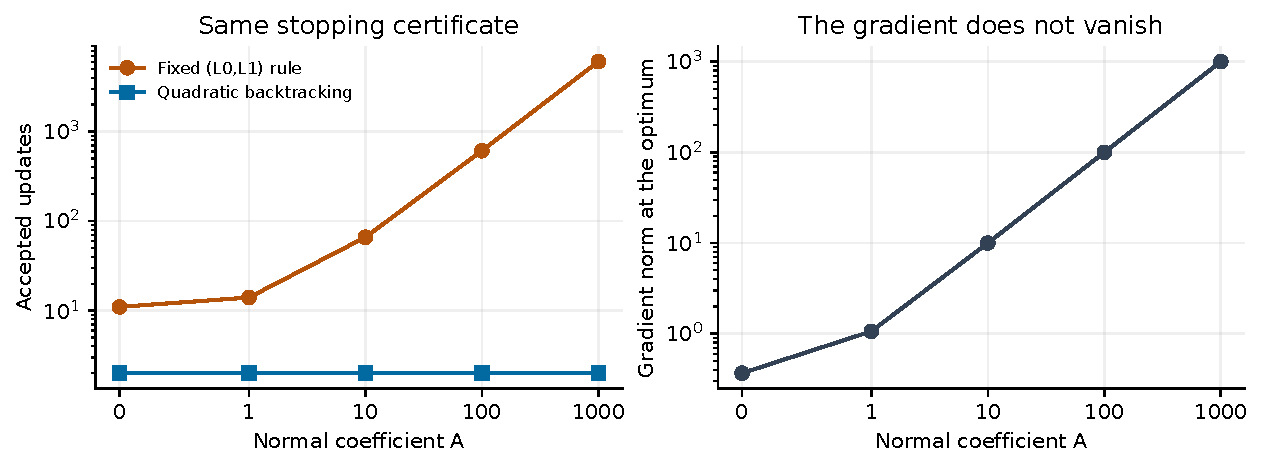
\includegraphics[width=\linewidth]{../figures/boundary_normal_benchmark.pdf}
\caption{Фиксированный шаг через норму градиента уменьшается с ростом
нормального коэффициента. Подбор шага выполняет те же два шага,
хотя градиент в минимуме неограниченно растёт.}
\label{fig:boundary}
\end{figure}

Скрипт \texttt{Code/benchmark\_boundary.py} сохраняет каждую посещённую
точку, зазор, накопленный сертификат, принятую кривизну и число
вызовов. Он проверяет допустимость точек, уменьшение функции,
аналитическую границу~\eqref{eq:normal_lower} и совпадение траекторий
подбора шага. Известное решение используется только для контрольной
проверки после остановки. Алгоритм не получает ни минимизатор,
ни значение минимума. В эксперименте используется арифметика Python
с плавающей точкой; утверждения разделов~\ref{sec:stopping}
и~\ref{sec:normal} доказаны независимо от численных проверок.

\paragraph{Смысл результата.}
Полный зазор даёт корректную остановку в граничном минимуме.
Подбор шага не зависит от нормального коэффициента в семействе из
утверждения~\ref{prop:normal_invariance}. В таблице~\ref{tab:boundary}
использован фиксированный Algorithm~1 работы~\cite{vyguzov};
доказательство и таблица относятся к одному и тому же сравнению.

\paragraph{Вычислительные инструменты.}
Инструменты ИИ использовались при выводах, проверках, подготовке кода
и текста. За проверку математических утверждений, источников и
вычислений отвечают авторы.
